% LaTeX2e Template by Stephen Iota (https://stepheniota.com/)
% last updated: Jan. 2019

% for papers
%\documentclass[aps,onecolumn,superscriptaddress]{revtex4-1}
% https://www-d0.fnal.gov/Run2Physics/WWW/templates/revtex4.pdf
% https://cdn.journals.aps.org/files/revtex/auguide4-1.pdf
% for revTeX4-1 class options

% for other
\documentclass[10pt]{article}
\usepackage[margin=3cm]{geometry}

%%%%%%%%%%%%%%%%
%%% Packages %%%
%%%%%%%%%%%%%%%%

\usepackage[utf8]{inputenc}
\usepackage{amsmath}
\usepackage{amssymb}
\usepackage{amsfonts} % to remove math font when typesetting equations
\usepackage[thinc]{esdiff} 
\usepackage{graphicx}
\usepackage[shortlabels]{enumitem} % to change labels in enum/item
\usepackage[dvipsnames]{xcolor} % for colored links

% always put this at the end
\usepackage[
	colorlinks=true,
	citecolor=green!50!black,
	linkcolor=NavyBlue!75!black,
	urlcolor=green!50!black,
	hypertexnames=false]{hyperref} 

 
 %%%%%%%%%%%%%%%%%%
 %% New Commands %%
 %%%%%%%%%%%%%%%%%%
 
\newcommand{\email}[1]{\texttt{\href{mailto:#1}{#1}}}

\newcommand{\hint}[1]{\color{Blue}{#1}}
 
%----------------------------------------------------
%%%%%%%%%%%%%%%%%%
%% Front Matter %%
%%%%%%%%%%%%%%%%%%

\pagenumbering{gobble} % no page numbers
\graphicspath{{figures/}} % set directory for figures
%\usepackage{wrapfig}
%\setcounter{section}{-1} % start with section 0

%%%%%%%%%%%%%
%%% Title %%%
%%%%%%%%%%%%%
\begin{document}

\begin{center}

\Large{\textsc{Week 5}: \textbf{Newton's 3rd Law}}

\end{center}

\vspace{.5mm}


%%%%%%%%%%
%% INFO %%
%%%%%%%%%%

\begin{tabular}{rl}
\textsc{SI Leader}:
&
Stephen Iota (\email{siota001@ucr.edu})
\\
\textsc{Course}:
&
Physics 40A (Winter 2019), Prof.~Ellison
\\
\textsc{Date}:
&
4 February 2019
\end{tabular}

%%%%%%%%%%%%%%
%% PROBLEMS %%
%%%%%%%%%%%%%%

\section{Warm-up}
\begin{enumerate}[(a)]
	\item What in what direction does the block to the right accelerate?
	\begin{center}
	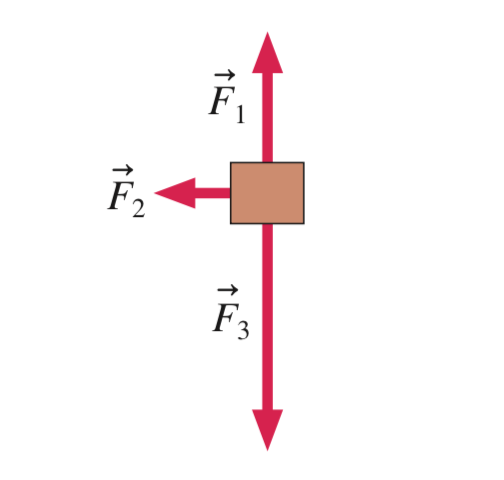
\includegraphics[width=.2\linewidth]{PS5-FigA}
	\end{center}
	\item What does Newton's 3rd Law say?
\end{enumerate}


\section{Action-Reaction Pairs}
\begin{enumerate}
	


\item All three 50 kg blocks are at rest. Is the tension in rope 2 greater than, less than, or equal to the tension in rope 1?
	\begin{center}
	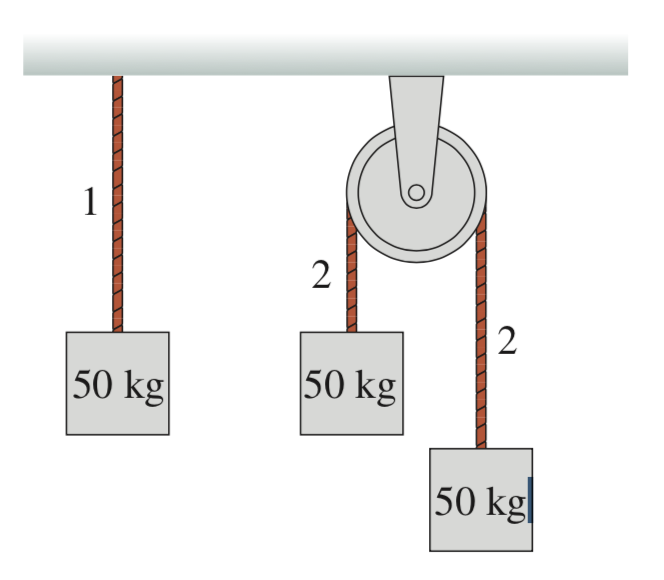
\includegraphics[width=.2\linewidth]{PS5-FigB}
 \end{center}
\item The hand in the figure belox pushed boxes A and B to the right across a frictionless table. The mass of B is larger than the mass of A.
 
\begin{enumerate}[(a)]
	\item Draw free-body diagrams of A, B, and hand H, showing only the horizontal forces.
	\item Rank in order, from larges to smallest, the horizontal forces shown on your free-body diagrams. 
\end{enumerate}

\begin{center}
	
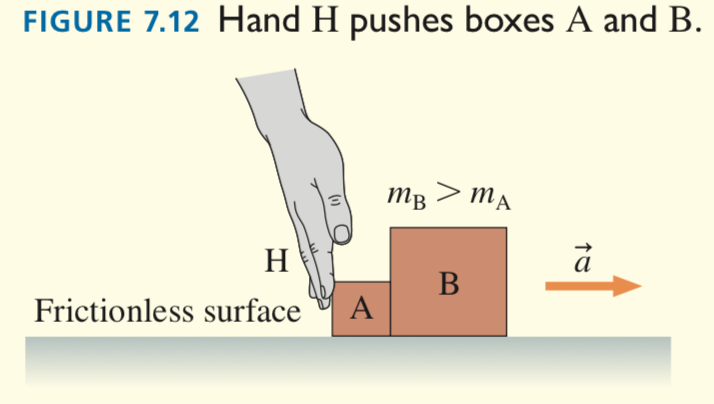
\includegraphics[width=.2\linewidth]{PS5-FigC}
\end{center}


\end{enumerate}

\section{Recoil Speed}
Bob, who has a mass of 75 kg, can throw a 500g rock with a speed of 30 m/s. The distance through which his hand moves as he accelerates the rock from rest until he releases it is 1.0 m.

\begin{enumerate}[(a)]
	\item What constant force must Bob exert on the rock to throw it with this speed?
	
	\item If bob is standing on frictionless ice, what is his recoil speed after releasing the rock?
	
\end{enumerate}
\end{document}